\chapter{Signal Extraction with Boosted Decision Trees}
\label{chap:BDT}

A \ac{MVA} is performed in \ac{SR} to further separate the LFV signals from the backgrounds, and enhance the sensitivity of this analysis. More specifically, a dozen of discriminating variables, referred to as ``features'', are selected and combined by a gradient-\ac{BDT}, which is implemented using the \textsc{XGBoost} package \cite{Chen:2016:XST:2939672.2939785}. There are several reasons why \ac{BDT} is chosen: (i) the goal of the \ac{MVA} is to achieve maximum separation between signals and backgrounds using a small number of already well-separated kinematic variables, instead of exploring some complicated structures hidden in event topology, (ii) under such a goal, the potential performance gain from a more sophisticated algorithm like a \ac{NN} is limited, (iii) a \ac{BDT}-based algorithm is straightforward to implement and consumes only a moderate amount of computational resources, and (iv) the interpretability of a \ac{BDT}-based algorithm is excellent. 

The top production and decay signals are longer distinguished by the \ac{BDT}. They are combined into a single signal class, just like all backgrounds are combined into a single background class. The training of the \ac{BDT} depends entirely on \ac{MC} samples that are statistically orthogonal to the samples used in the actual background estimation. More details on the configurations of the \ac{BDT} are described in \autoref{sec:Config}. The input features are described in \autoref{sec:Input}. The output of the \ac{BDT} is presented in \autoref{sec:Output}.
%%%%%%%%%%%%%%%%%%%%%%%%%%%%%%%%%%%%%%%%%%%%%%%%%%%%%%%%%%
%%%%%%%%%%%%%%%%%%%%%%%%%%%%%%%%%%%%%%%%%%%%%%%%%%%%%%%%%%

\section{BDT Configuration}
\label{sec:Config}

Since the kinematic distributions of final state particles in our two signal channels (single top production and top decay) differ significantly (see Figure \ref{fig:Features1}-\ref{fig:Features5}), the SR is divided into two parts (SR1: $M_{e\mu}\leq$150GeV; SR2: $M_{e\mu}>$150GeV) in order to achieve the optimal sensitivity. Within each sub-region of the SR, a binary BDT is trained.
   
The signal datasets used for BDT training are MC samples that correspond to single top LFV production (ST) and top LFV decay (TT). The Lorentz structure and the flavor of the up-type quark involved in LFV interaction were shown to have a minor impact on the kinematics of final state particles (See Figure~\ref{fig:Lorentz}). Therefore, they were not further distinguished.  

\begin{figure}[tbh!]
 \begin{center}
 \begin{tabular}{cc}
  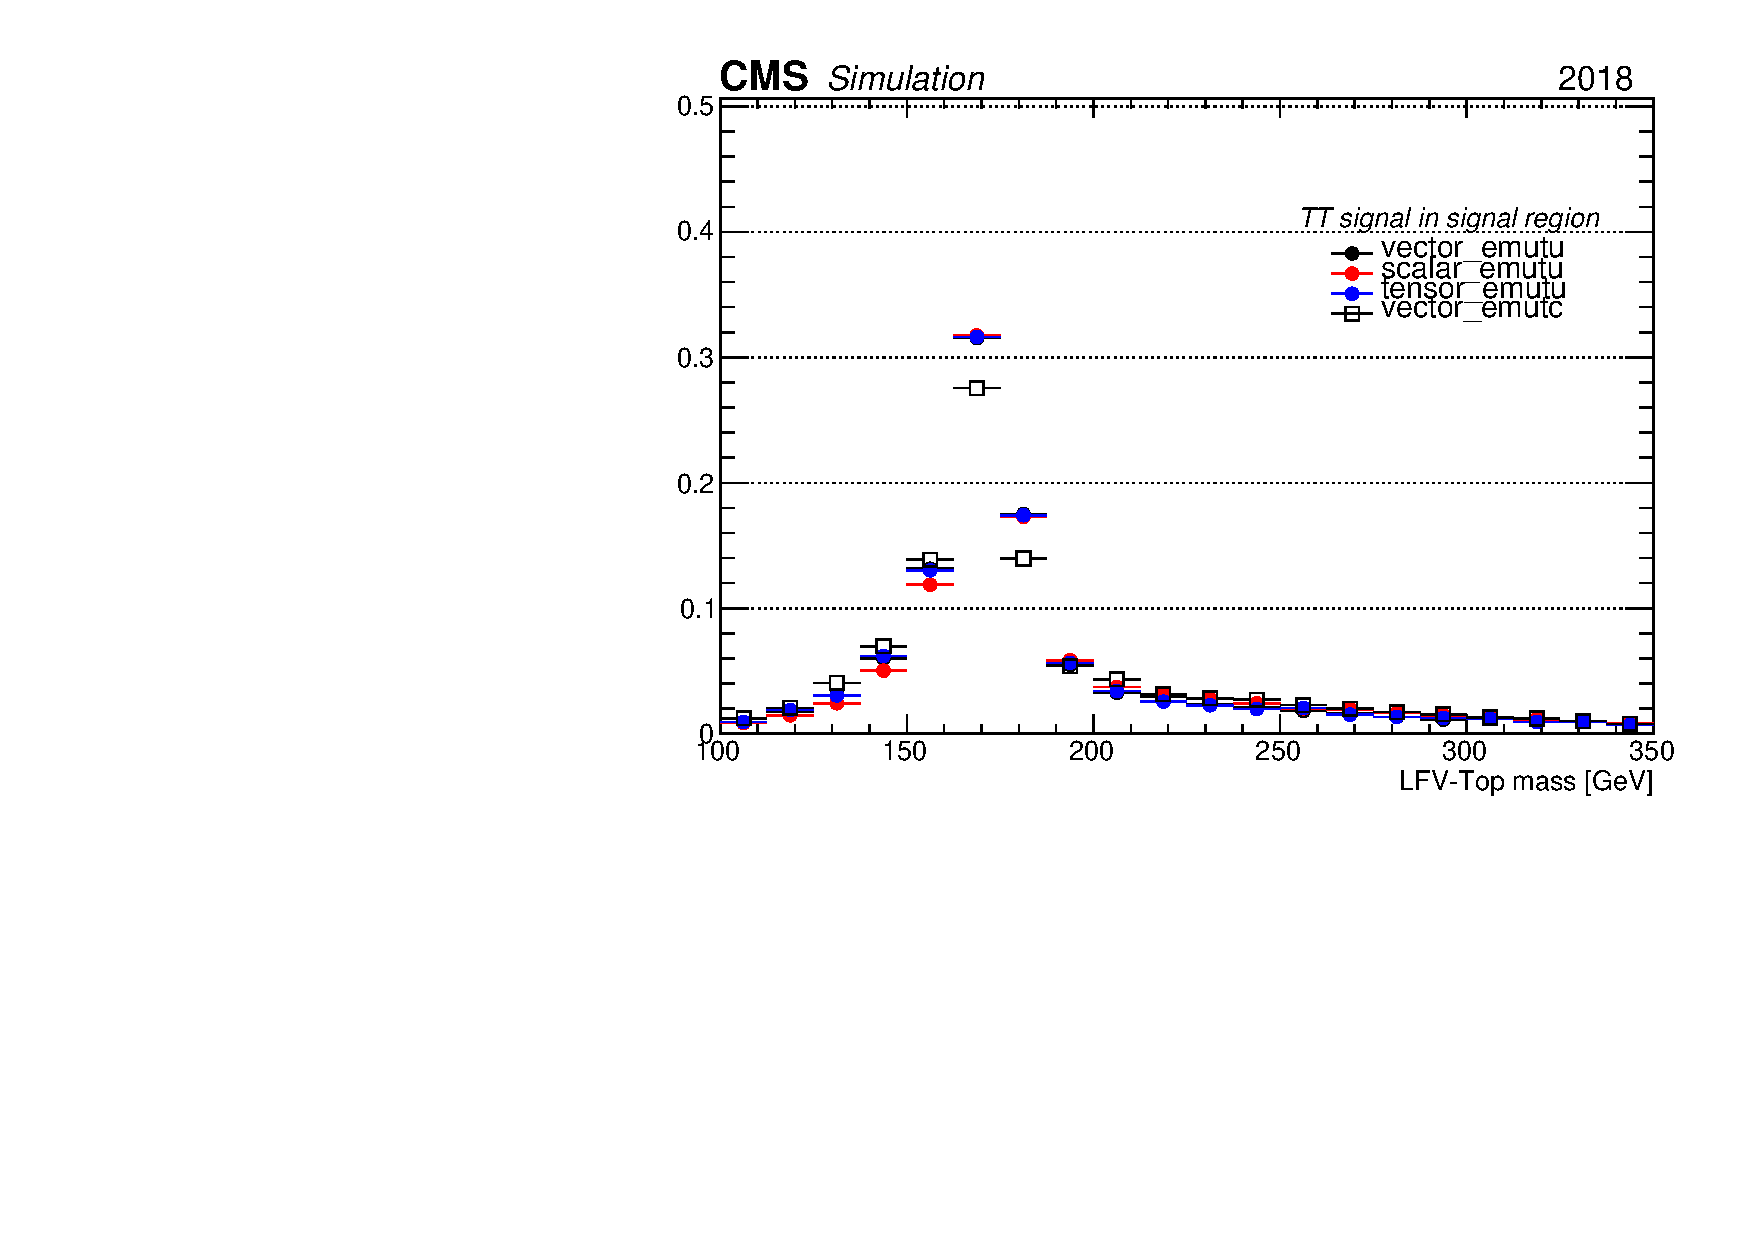
\includegraphics[width=0.48\textwidth]{figures/Part3/BDT/LFV_VR_emul_lllOffZMetg20Jetgeq1Bleq1_LFVTopmass_N}&
    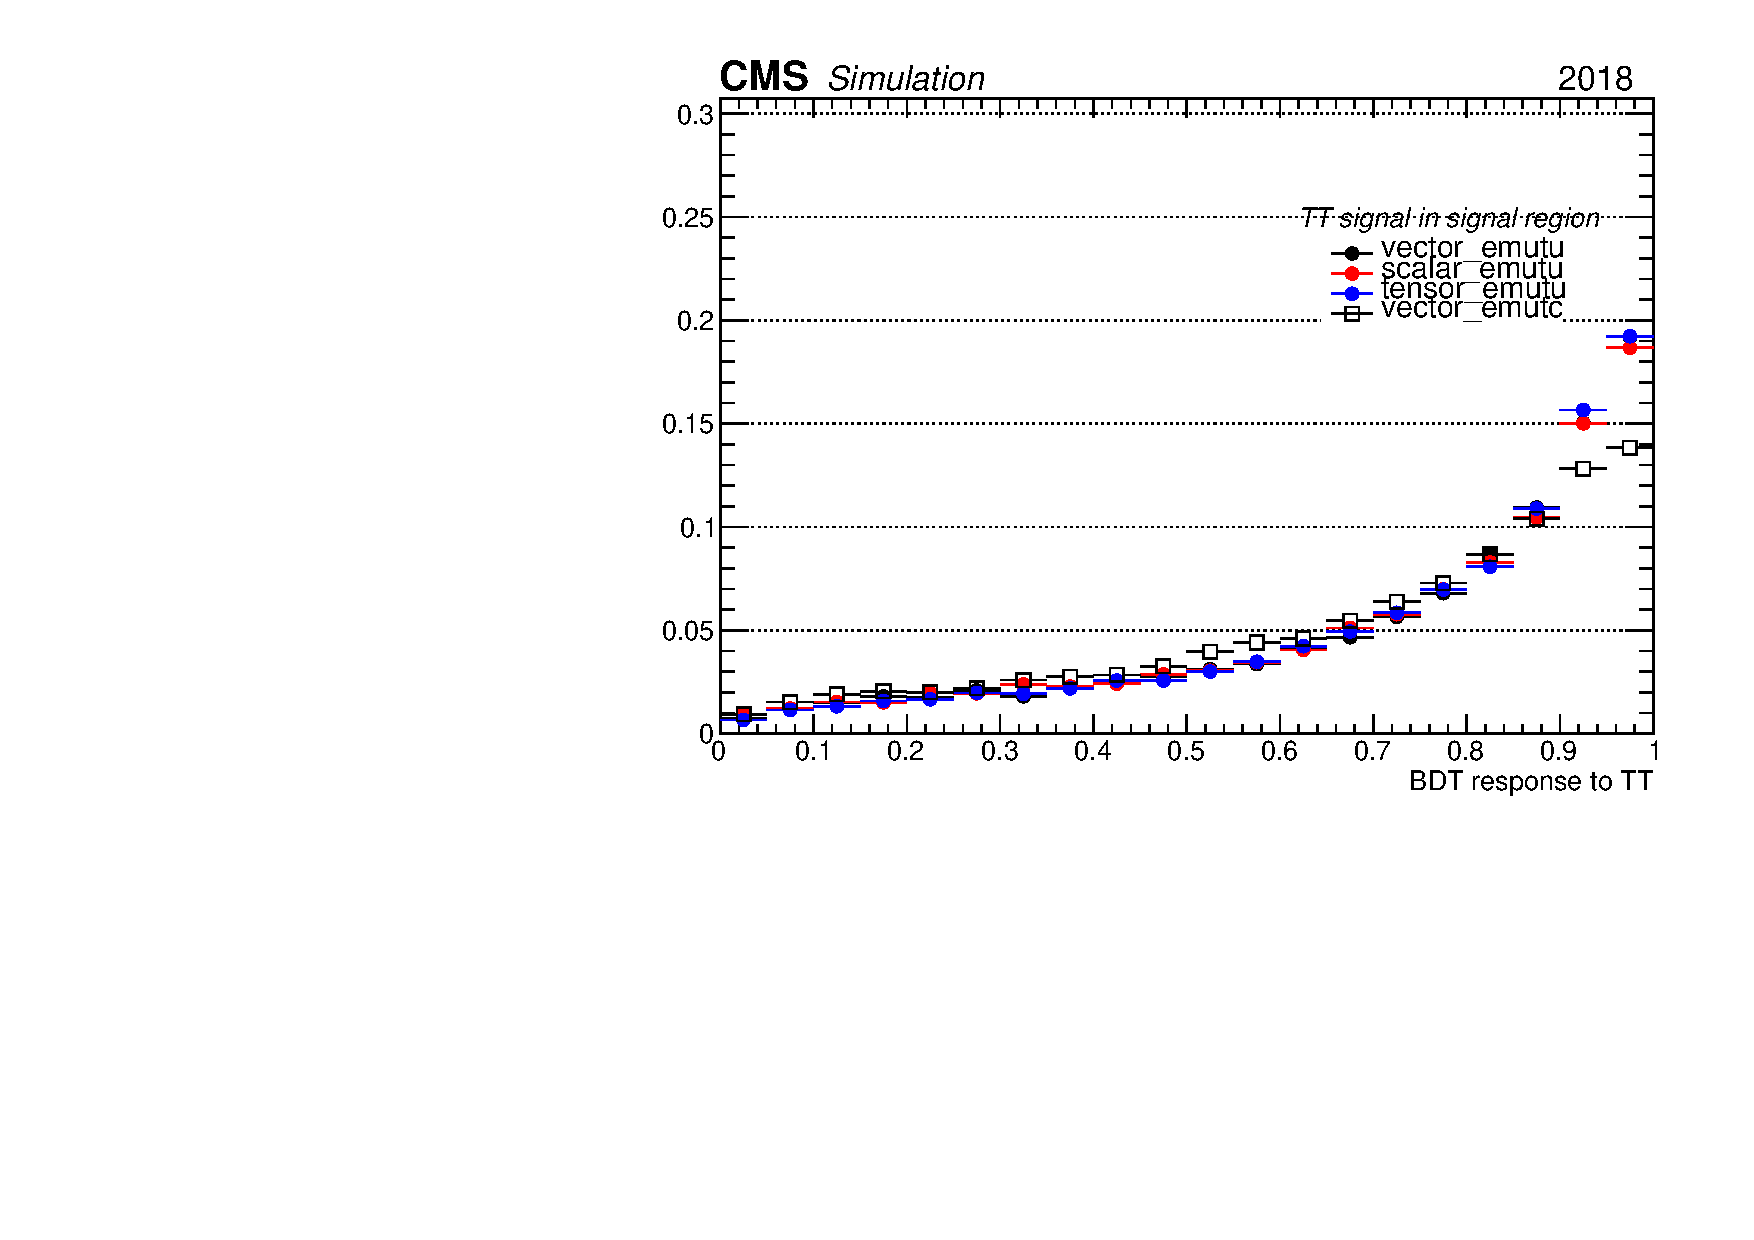
\includegraphics[width=0.48\textwidth]{figures/Part3/BDT/LFV_VR_emul_lllOffZMetg20Jetgeq1Bleq1_BDT_TT_N}\\
 \end{tabular}
 \caption{Normalized distribution in SR1. From left to right: LFV top mass, BDT shape}
 \label{fig:Lorentz}
 \end{center}
\end{figure}

The background MC samples include all the samples listed in Table \ref{tab:2016MCsample}-\ref{tab:20172018MCsample}. It was determined that splitting the background into separate classes (prompt vs non-prompt backgrounds) did not increase the signal discrimination power and caused overtraining which is why in the backgrounds are combined. 

\begin{figure}[tbh!]
 \begin{center}
 \begin{tabular}{cc}
  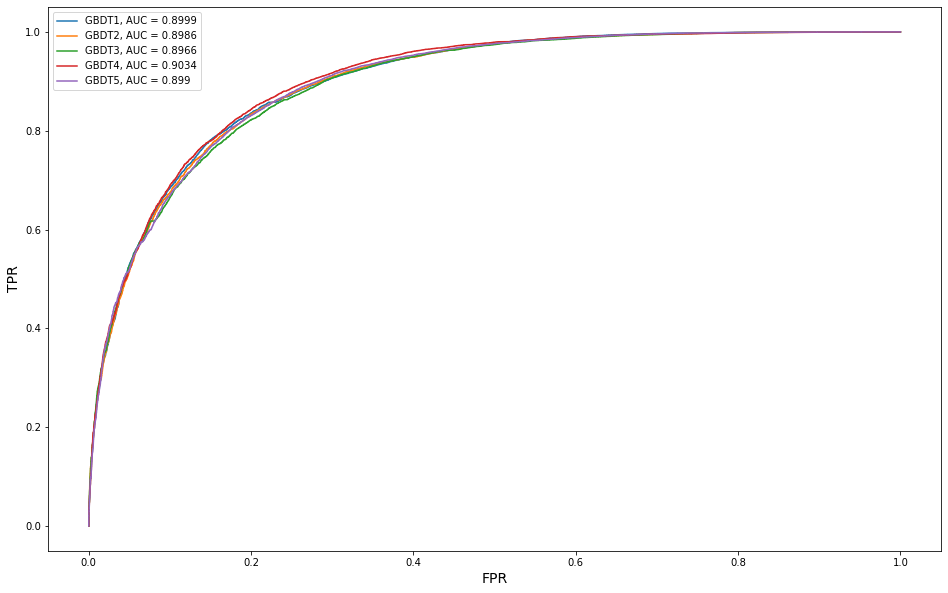
\includegraphics[width=0.48\textwidth]{figures/Part3/BDT/5foldTT}&
    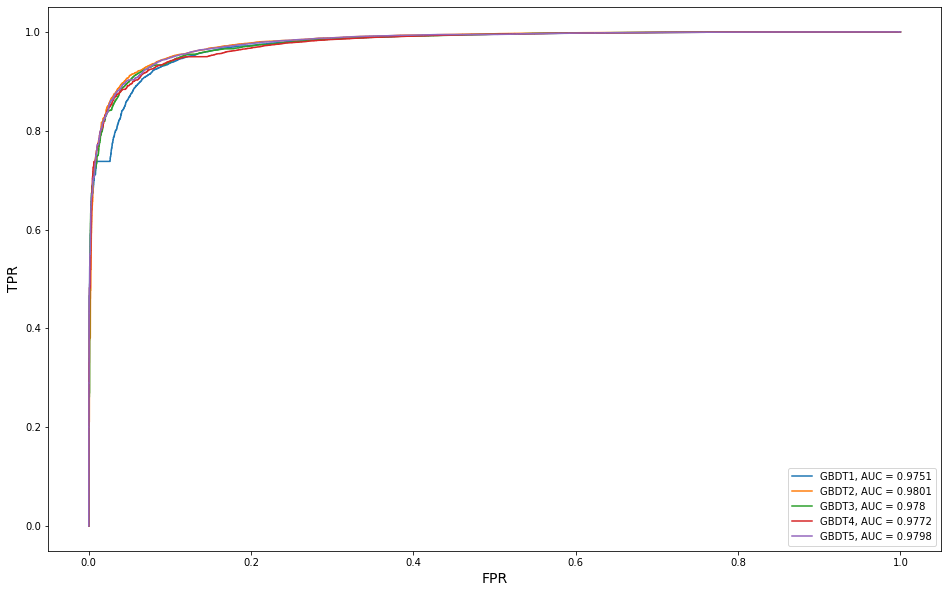
\includegraphics[width=0.48\textwidth]{figures/Part3/BDT/5foldST}\\
 \end{tabular}
 \caption{ROC curve with 5-fold cross validation. From left to right: BDT targeting TT (SR1), BDT targeting ST (SR2).}
 \label{fig:5fold}
 \end{center}
\end{figure}

The MC dataset is divided into 5 subsets evenly. A 5-fold cross-validation scheme is deployed: the training set consists of 3 out of the 5 subsets, while validation/testing set each consists of 1 subset. The number of estimators is set to 1000, max depth 5, and sub-sample 0.8 with the evaluation metric set to "mlogloss".  The results of the cross-validation study are shown in Figure \ref{fig:5fold}. The trained BDT model targeting TT(ST) signal is used to evaluate each event in SR1(SR2): a BDT weight is assigned to each event, giving the likelihood that it originated from TT(ST) signal. 
%%%%%%%%%%%%%%%%%%%%%%%%%%%%%%%%%%%%%%%%%%%%%%%%%%%%%%%%%%
%%%%%%%%%%%%%%%%%%%%%%%%%%%%%%%%%%%%%%%%%%%%%%%%%%%%%%%%%%

\section{BDT Features}
\label{sec:Input}

The observables used in training are referred to as "features" in this analysis. The following features are used for both ST and TT classifier:

\begin{itemize}
\item \textbf{MVA\_M$_{e\mu}$: invariant mass of the Opposite-Sign $e\mu$ pair}
\item \textbf{MVA\_LFVePt: $p_T$ of the flavor-violating electron}
\item \textbf{MVA\_LFVmuPt: $p_T$ of the flavor-violating muon}
\item \textbf{MVA\_LFVTopmass: invariant mass of the flavor-violating top-quark candidate}
\item \textbf{MVA\_Zmass: invariant mass of Z boson candidate}
\item \textbf{MVA\_Jet2Btag: b-tagging score of the jet with the second highest b-tagging score}
\item \textbf{MVA\_Mbl2: invariant mass of the second b-jet+lepton system}
\item \textbf{MVA\_njet: number of jets}
\item \textbf{MVA\_nbjet: number of b-jets}
\item \textbf{MVA\_tM: transverse mass of the W boson candidate (from standard model top-quark)}
\item \textbf{MVA\_llDr: $\Delta R$ between flavor-violating electron and muon}
\item \textbf{MVA\_SSee\_Zmass: invariant mass of a Same-Sign di-electron pair}
\item \textbf{MVA\_Topmass: invariant mass of the standard model top-quark candidate}
\item \textbf{MVA\_Met: missing transverse energy}
\end{itemize}

The following features are only used for TT classifier:

\begin{itemize}
\item \textbf{MVA\_Ht: scalar sum of the $p_T$ of all objects}
\item \textbf{MVA\_Mbl1: invariant mass of the second bjet+lepton system}
\item \textbf{MVA\_JeDr: $\Delta R$ between flavor-violating electron and a light jet (non-b-jet)}
\item \textbf{MVA\_JmuDr: $\Delta R$ between flavor-violating muon and a light jet (non-b-jet)}
\end{itemize}

The following features are used for ST classifier:

\begin{itemize}
\item \textbf{MVA\_BaPt: $p_T$ of the standard model lepton}
\item \textbf{MVA\_JetHt: scalar sum of the $p_T$ of jets}
\end{itemize}

Distributions of selected features are shown in Figure \ref{fig:Features1}-\ref{fig:Features5}.

\begin{figure}[tbh!]
 \begin{center}
 \begin{tabular}{c}
  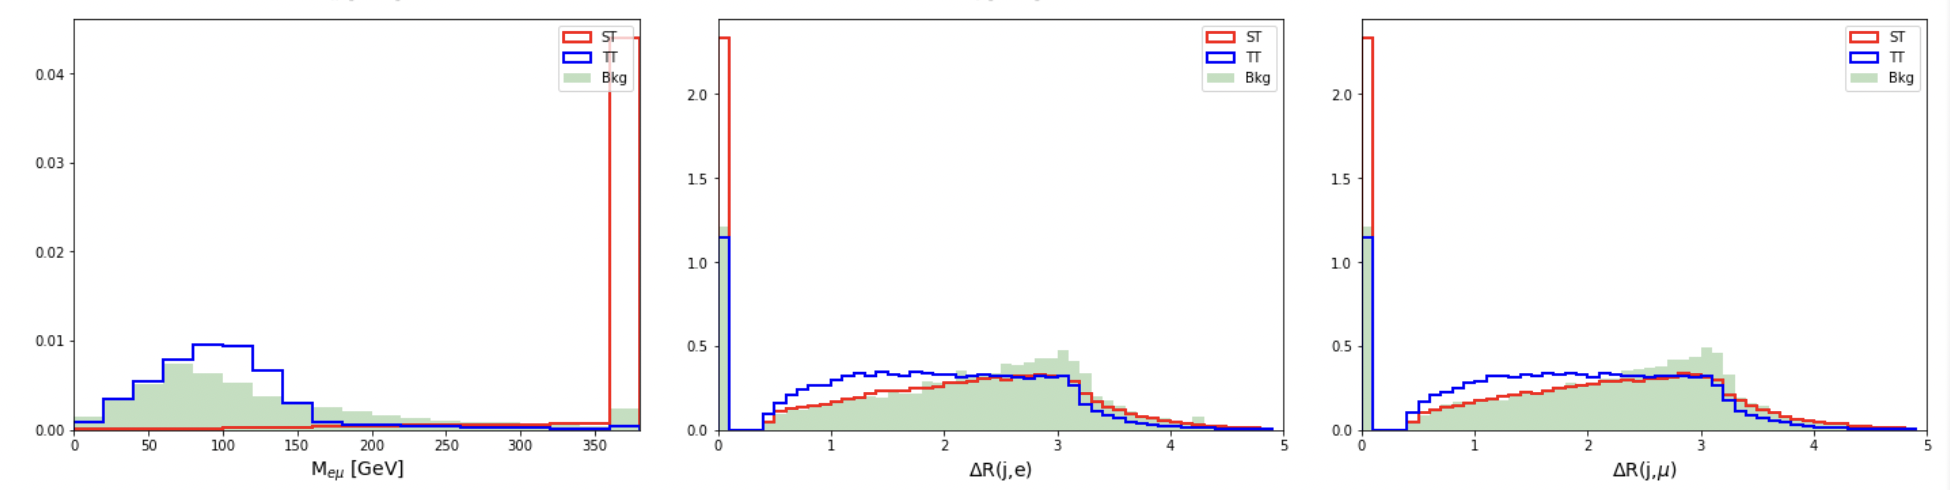
\includegraphics[width=0.99\textwidth]{figures/Part3/BDT/Features1}\\
 \end{tabular}
 \caption{Normalized distribution of various features in SR. From to left to right: MVA\_M$_{e\mu}$, MVA\_JeDr, MVA\_JeDr.}
 \label{fig:Features1}
 \end{center}
\end{figure}

\begin{figure}[tbh!]
 \begin{center}
 \begin{tabular}{c}
  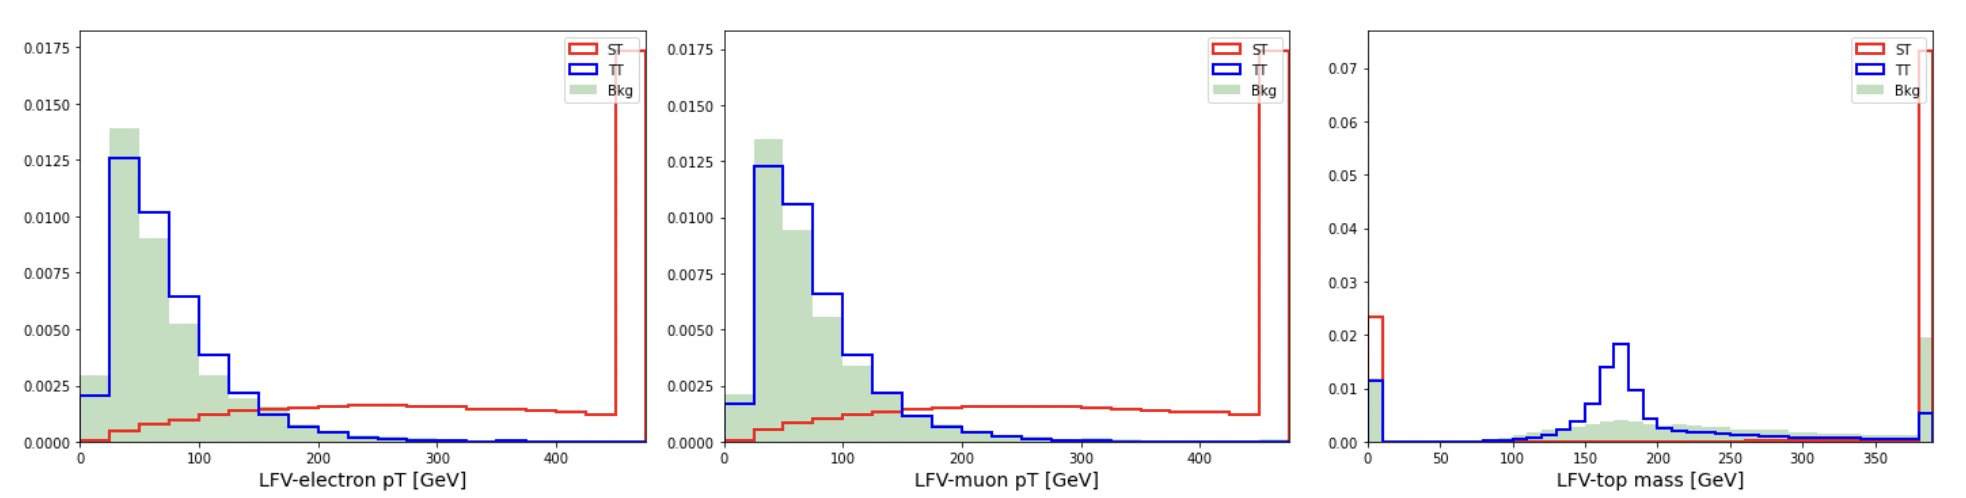
\includegraphics[width=0.99\textwidth]{figures/Part3/BDT/Features2}\\
 \end{tabular}
 \caption{Normalized distribution of additional features in SR. From to left to right: MVA\_LFVePt, MVA\_LFVmuPt, MVA\_LFVTopmass.}
 \label{fig:Features2}
 \end{center}
\end{figure}

\begin{figure}[tbh!]
 \begin{center}
 \begin{tabular}{c}
  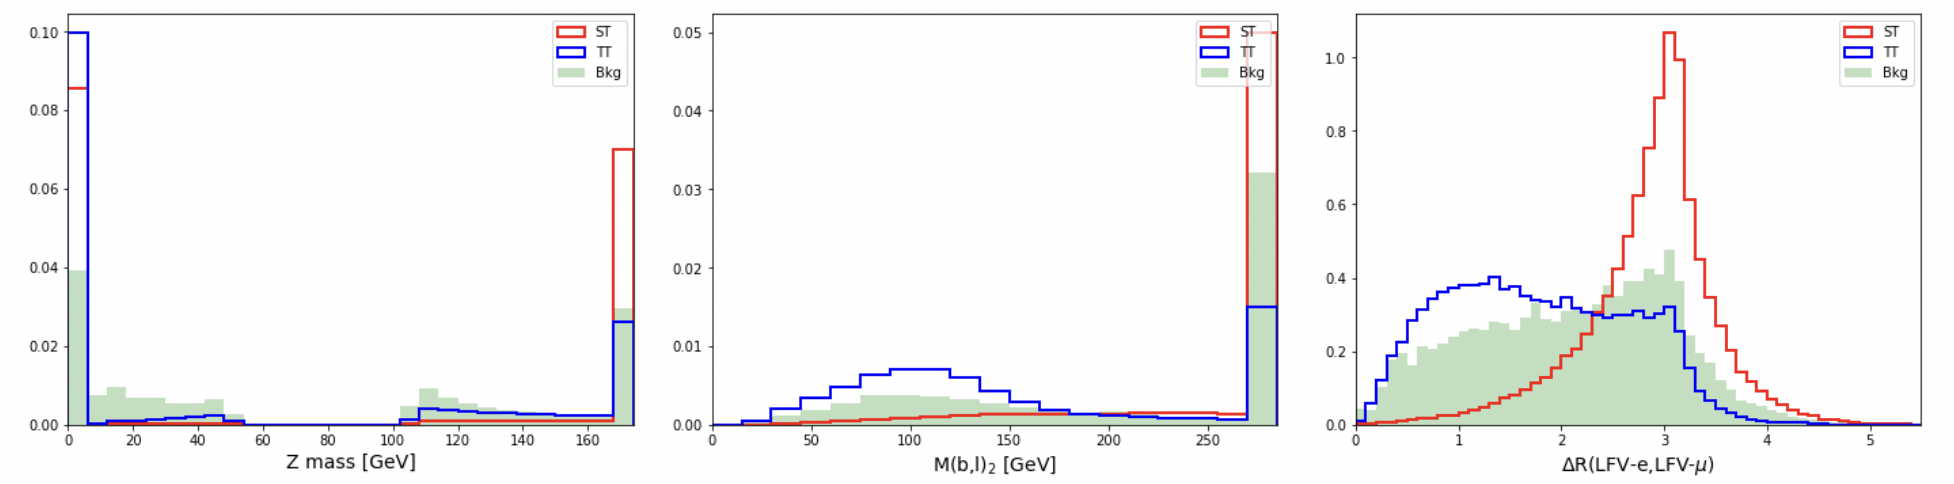
\includegraphics[width=0.99\textwidth]{figures/Part3/BDT/Features3}\\
 \end{tabular}
 \caption{Normalized distribution of additional features in SR. From to left to right: MVA\_Zmass, MVA\_Mbl2, MVA\_llDr.}
 \label{fig:Features3}
 \end{center}
\end{figure}

\begin{figure}[tbh!]
 \begin{center}
 \begin{tabular}{c}
  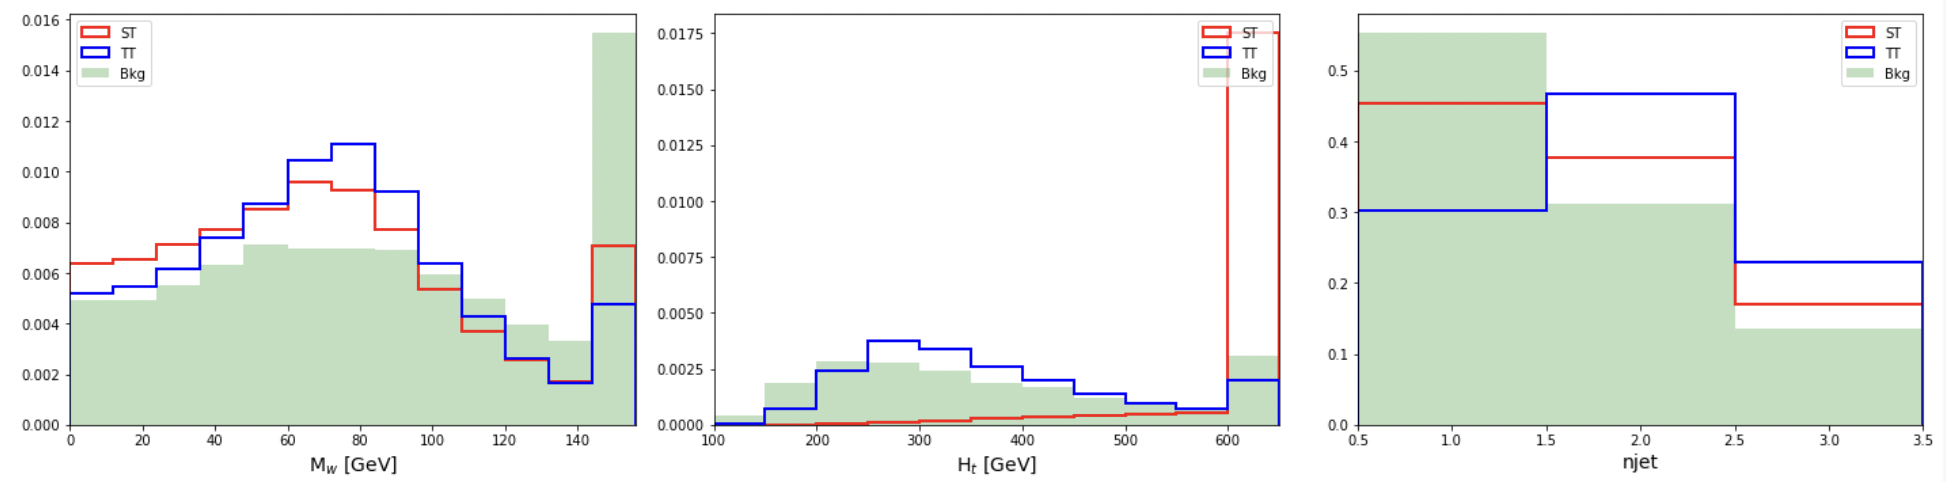
\includegraphics[width=0.99\textwidth]{figures/Part3/BDT/Features4}\\
 \end{tabular}
 \caption{Normalized distribution of additional features in SR. From to left to right: MVA\_tM, MVA\_Ht, MVA\_njet.}
 \label{fig:Features4}
 \end{center}
\end{figure}

\begin{figure}[tbh!]
 \begin{center}
 \begin{tabular}{c}
  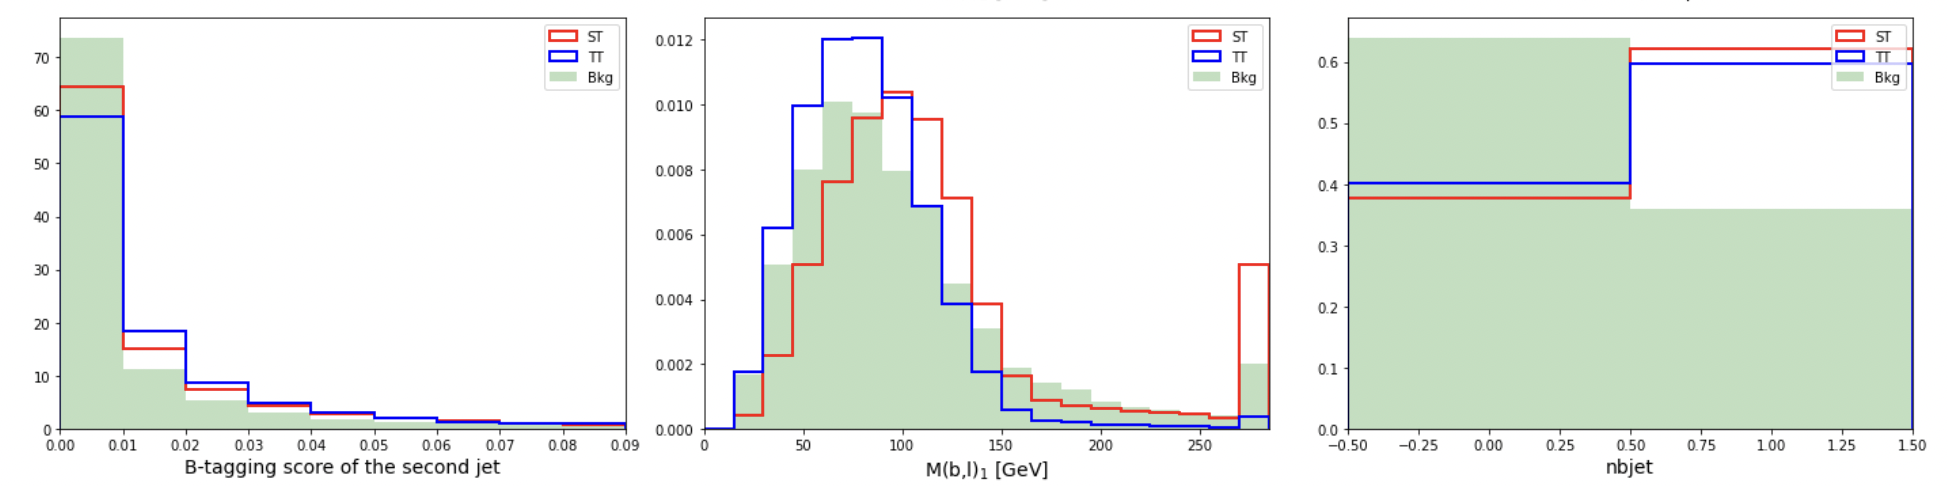
\includegraphics[width=0.99\textwidth]{figures/Part3/BDT/Features5}\\
 \end{tabular}
 \caption{Normalized distribution of additional features in SR. From to left to right: MVA\_Jet2Btag, MVA\_Mbl1, MVA\_nbjet.}
 \label{fig:Features5}
 \end{center}
\end{figure}

To determine the relative importance of these features, feature importance is extracted using the "gain" method and is shown in Figure \ref{fig:Ranking}.

\begin{figure}[tbh!]
 \begin{center}
 \begin{tabular}{cc}
  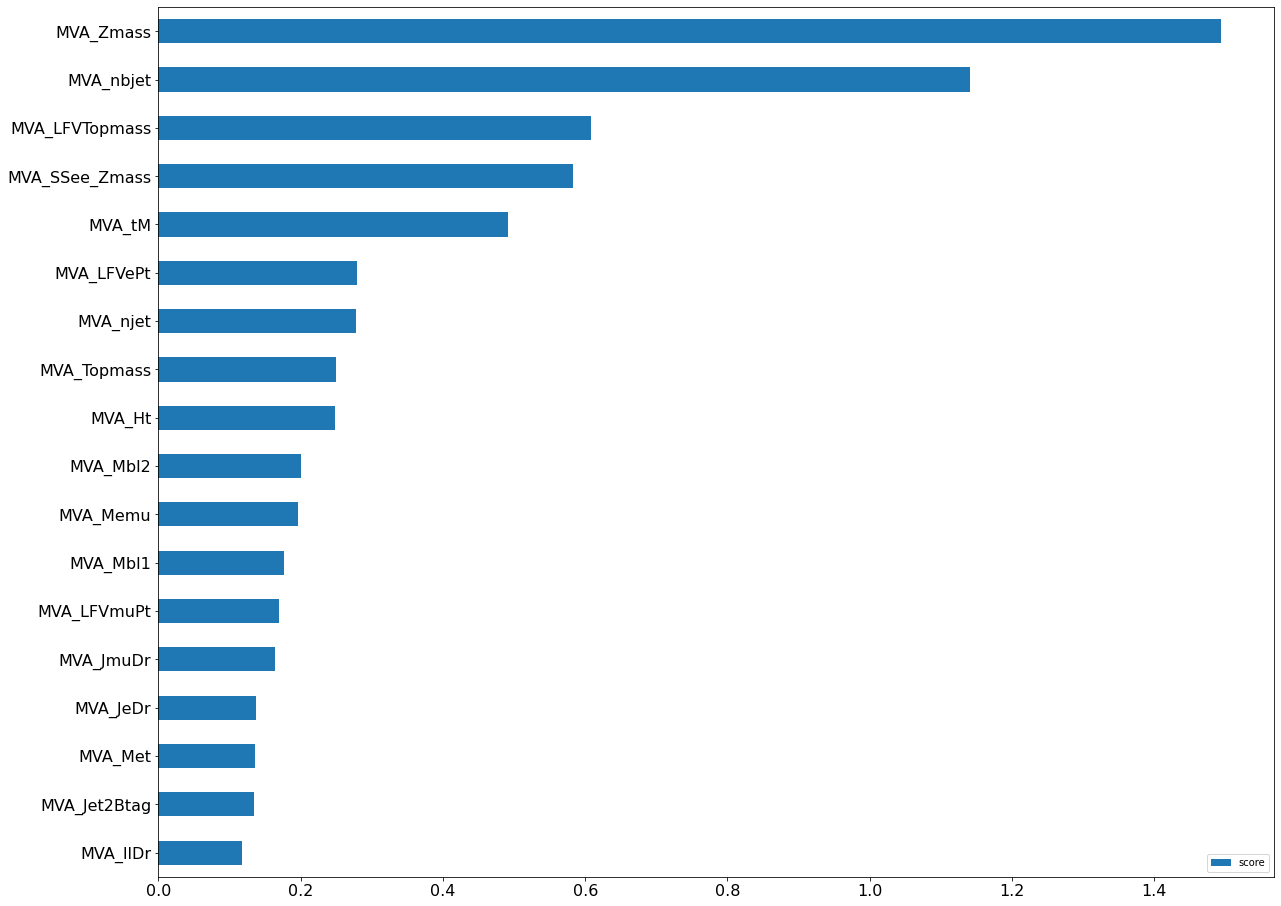
\includegraphics[width=0.48\textwidth]{figures/Part3/BDT/TTranking}&
  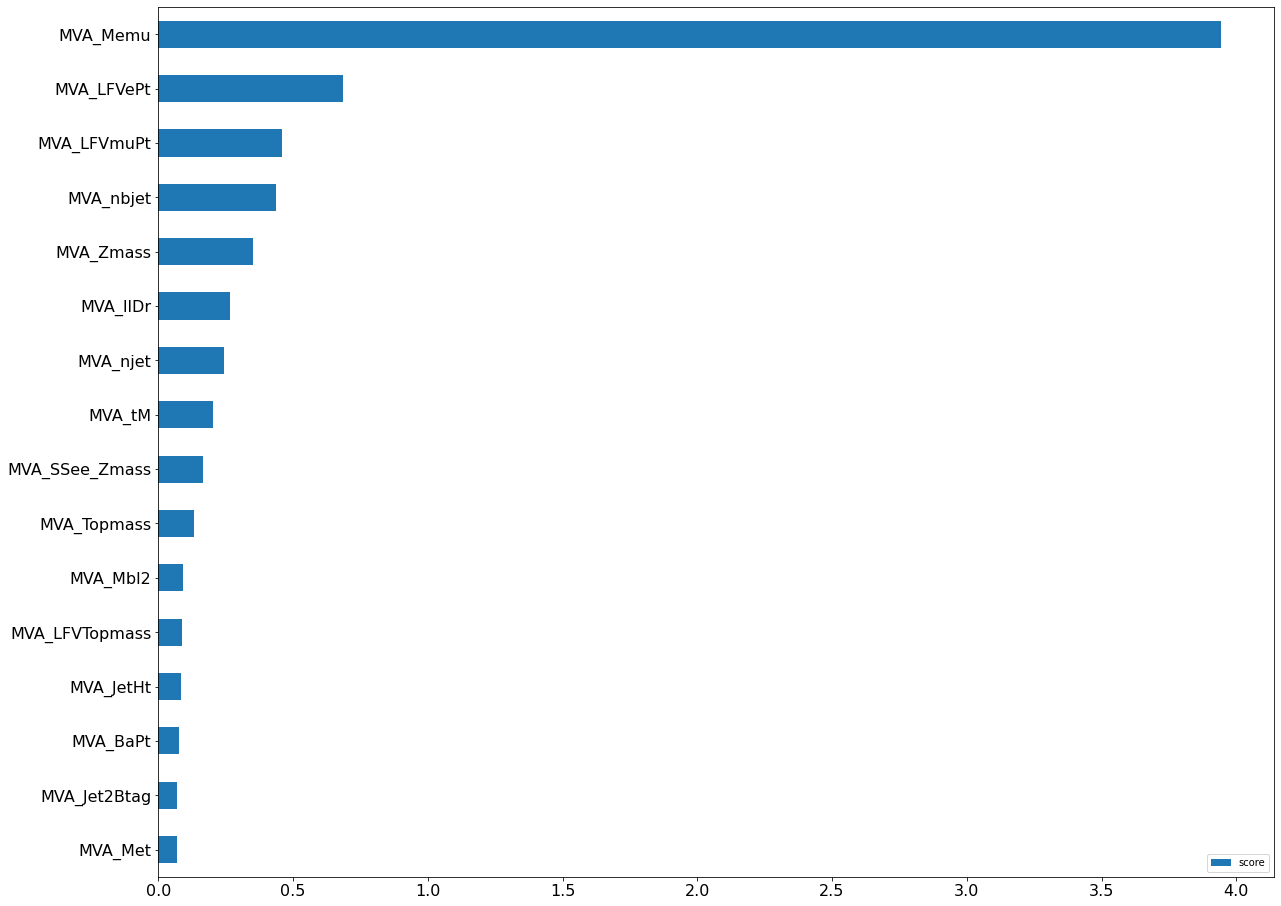
\includegraphics[width=0.48\textwidth]{figures/Part3/BDT/STranking}\\
 \end{tabular}
 \caption{List of features ranked by their relative importance. From left to right: BDT targeting TT (SR1), BDT targeting ST (SR2)}
 \label{fig:Ranking}
 \end{center}
\end{figure}

\begin{figure}[tbh!]
 \begin{center}
 \begin{tabular}{cc}
  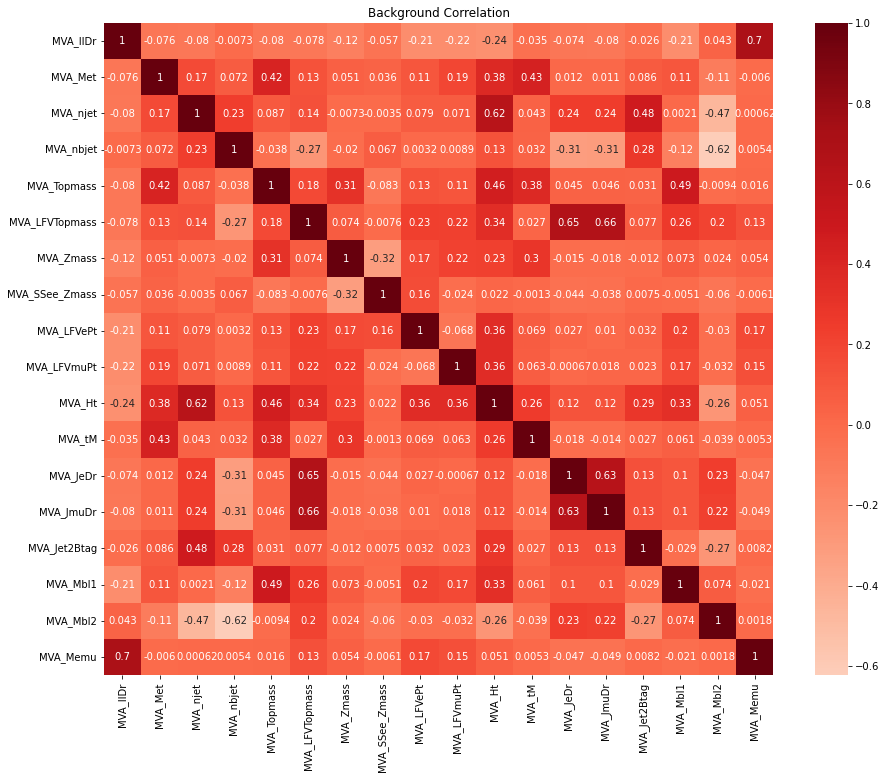
\includegraphics[width=0.48\textwidth]{figures/Part3/BDT/corr_bkg_SR1}&
  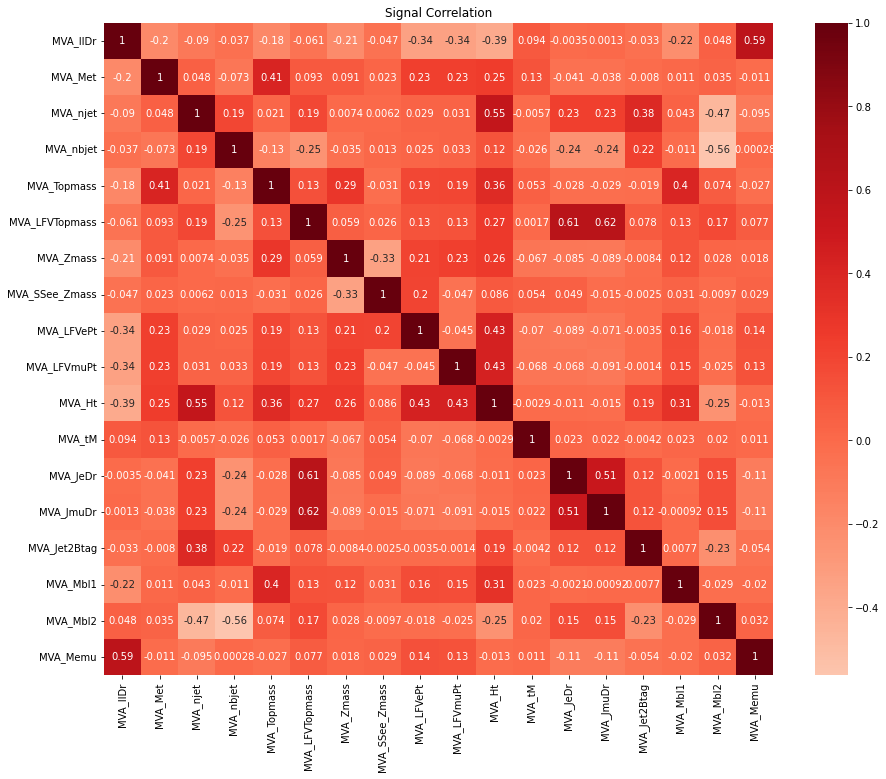
\includegraphics[width=0.48\textwidth]{figures/Part3/BDT/corr_signal_SR1}\\
 \end{tabular}
 \caption{Correlation matrices (SR1), from left to right: background correlation, signal correlation.}
 \label{fig:Ranking}
 \end{center}
\end{figure}

\begin{figure}[tbh!]
 \begin{center}
 \begin{tabular}{cc}
  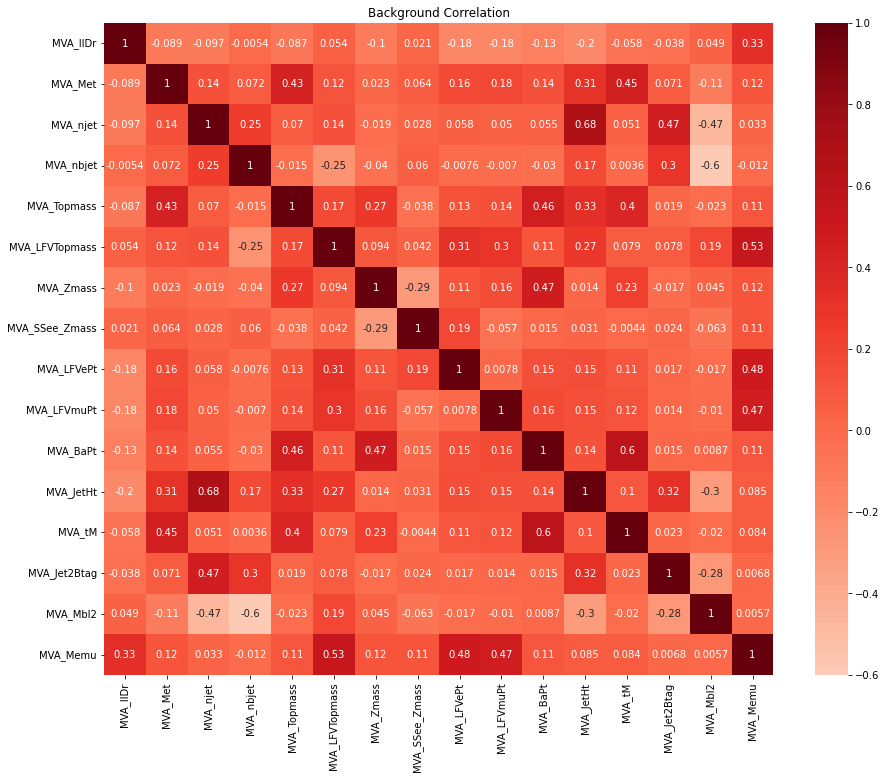
\includegraphics[width=0.48\textwidth]{figures/Part3/BDT/corr_bkg_SR2}&
  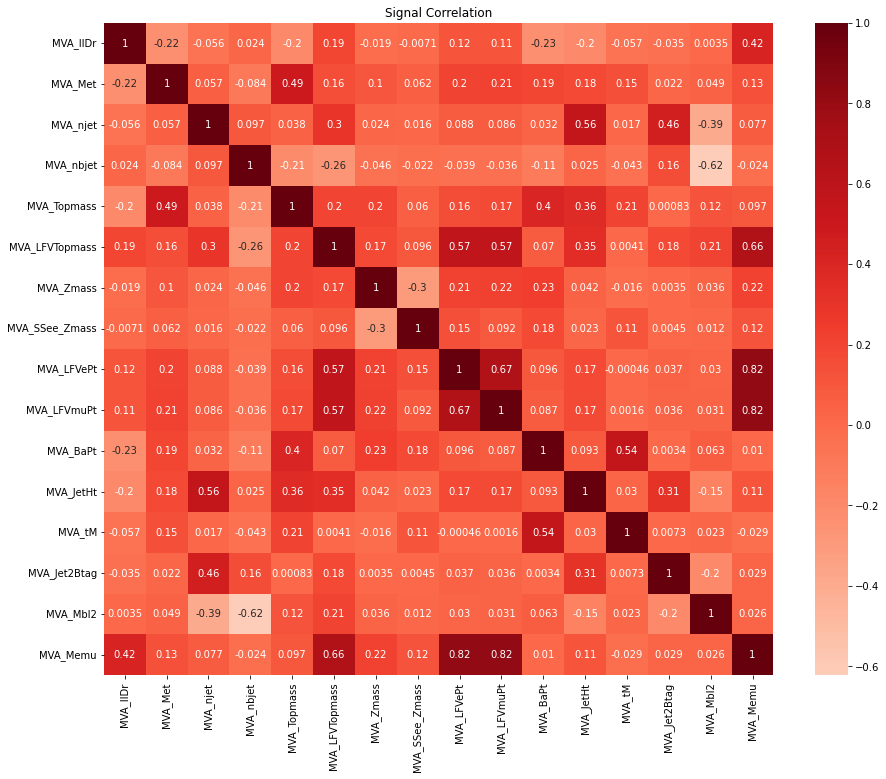
\includegraphics[width=0.48\textwidth]{figures/Part3/BDT/corr_signal_SR2}\\
 \end{tabular}
 \caption{Correlation matrices (SR2), from left to right: background correlation, signal correlation.}
 \label{fig:Ranking}
 \end{center}
\end{figure}
%%%%%%%%%%%%%%%%%%%%%%%%%%%%%%%%%%%%%%%%%%%%%%%%%%%%%%%%%%
%%%%%%%%%%%%%%%%%%%%%%%%%%%%%%%%%%%%%%%%%%%%%%%%%%%%%%%%%%

\section{BDT Output}
\label{sec:Output}

The output of the BDTs are shown in Figure \ref{fig:bdt_output}. Note: all but the nonprompt backgrounds are estimated with MC simulation. The nonprompt background backgrounds are estimated with the matrix method.

\begin{figure}[tbh!]
 \begin{center}
 \begin{tabular}{cc}
  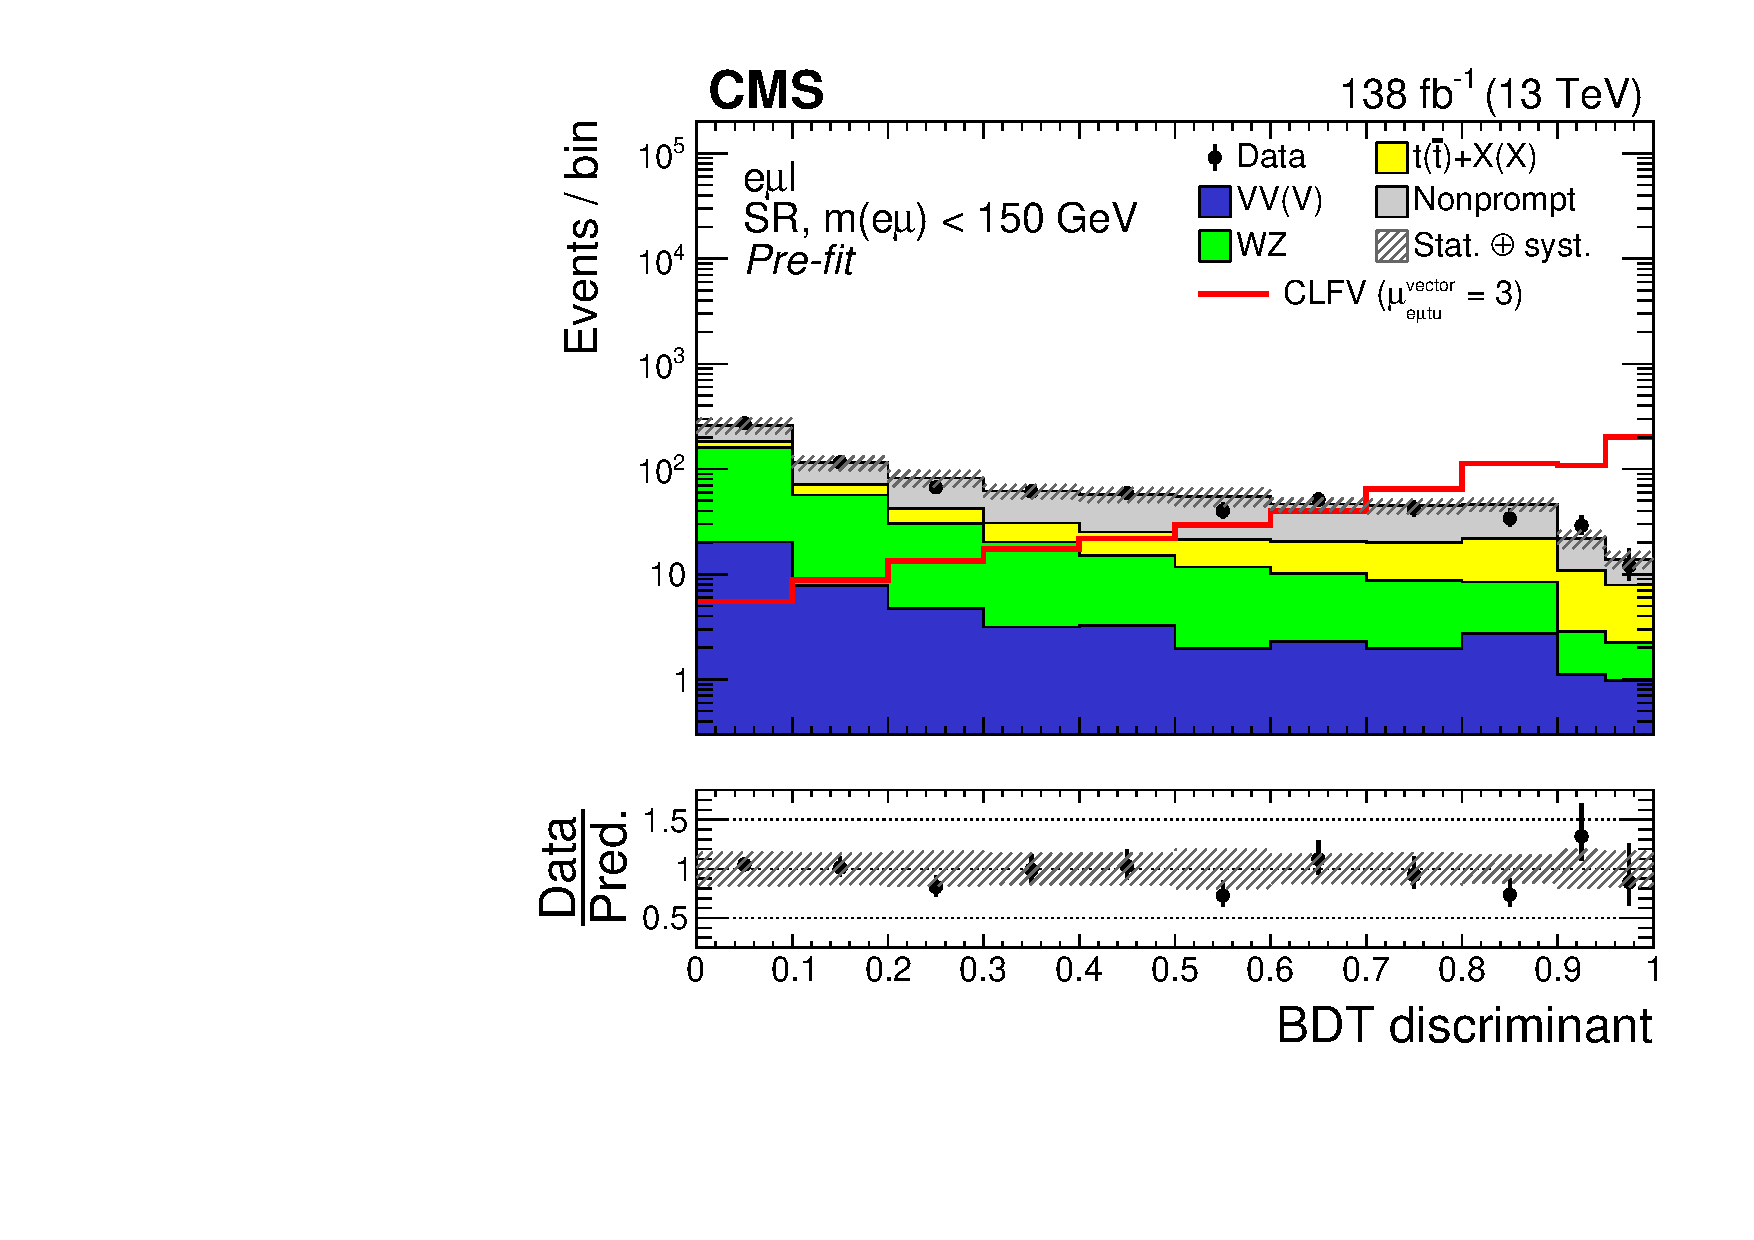
\includegraphics[width=0.48\textwidth]{figures/Part3/BDT/BDT_TT}&
  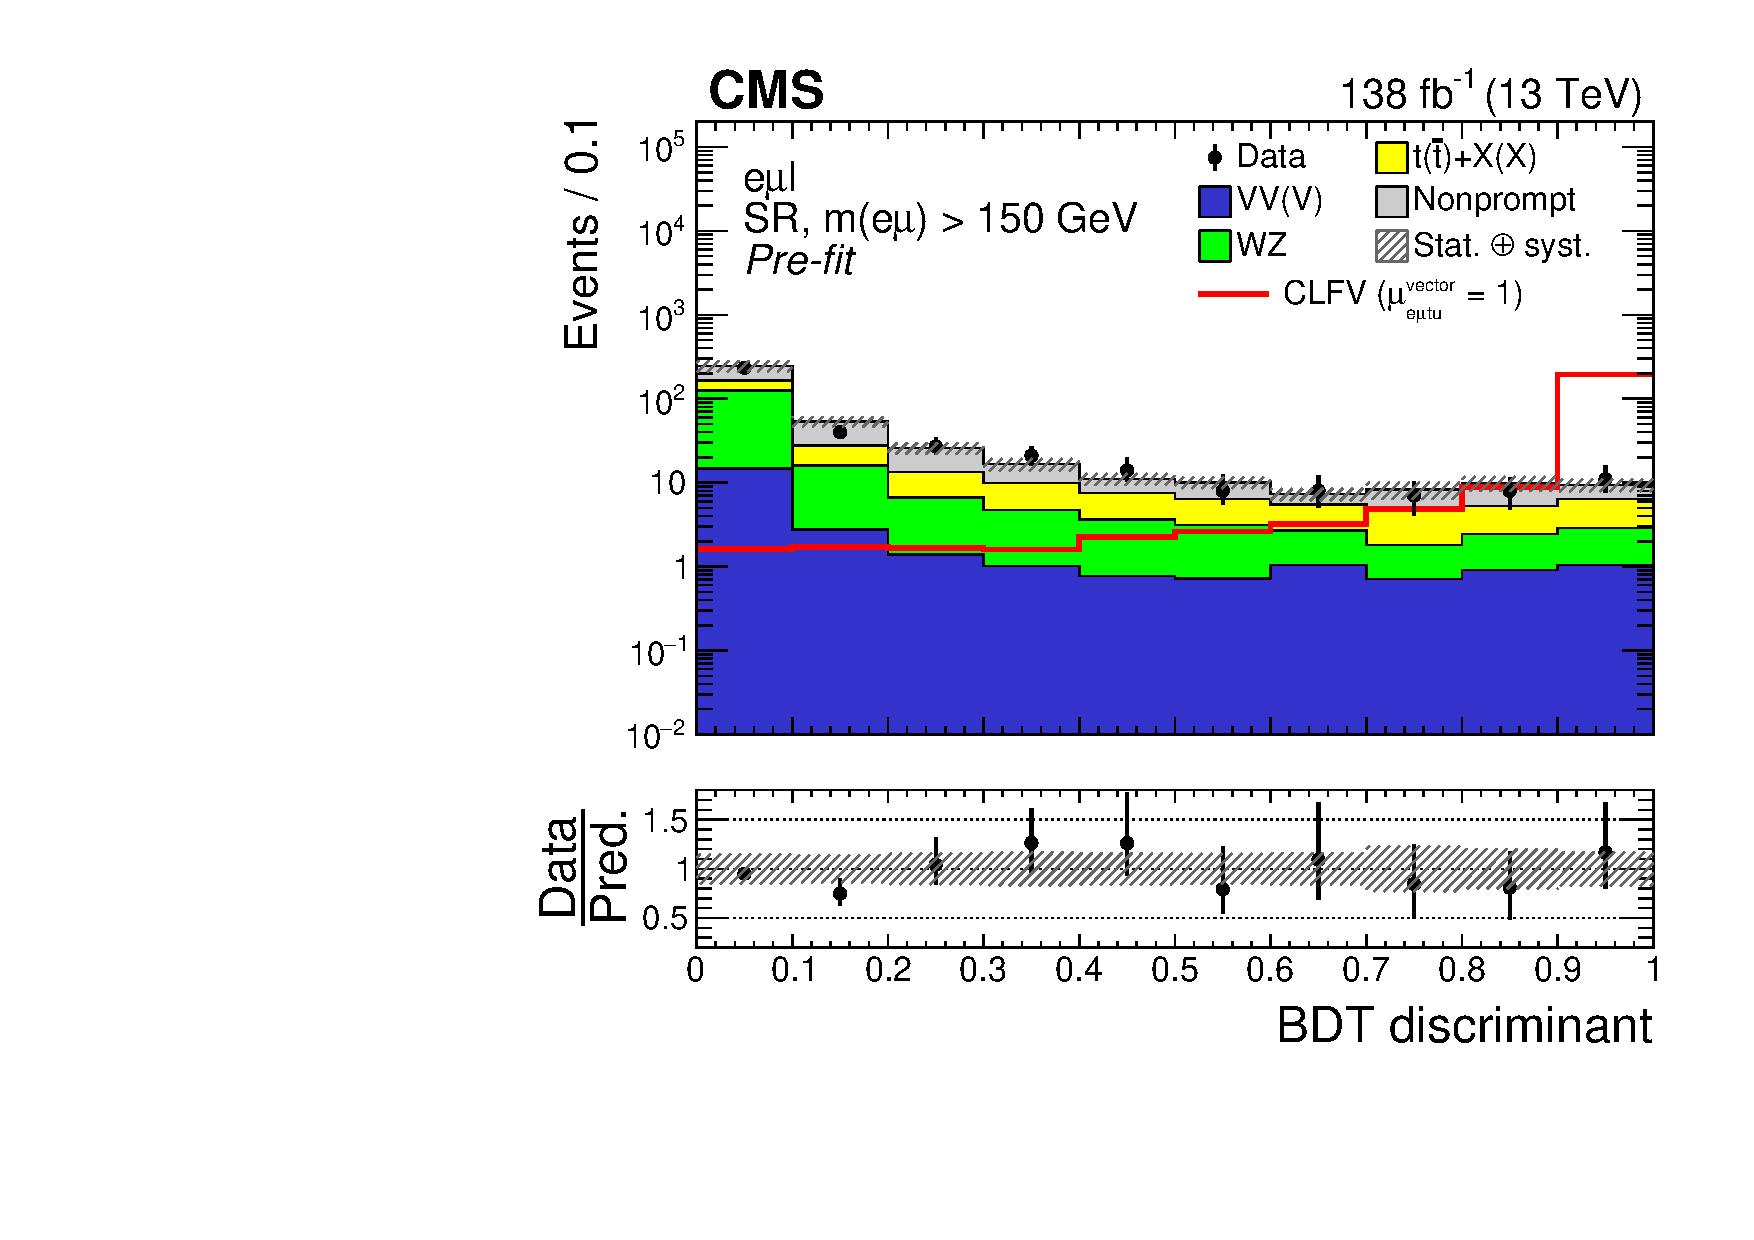
\includegraphics[width=0.48\textwidth]{figures/Part3/BDT/BDT_ST}\\
 \end{tabular}
 \caption{Distribution of BDT output, from left to right TT enriched SR (SR1), ST enriched SR (SR2)}
 \label{fig:bdt_output}
 \end{center}
\end{figure}